%===================================== CHAP 2 =================================

\chapter{Literature Review} \label{chp:litterature} 
This project's objective is to identify the underlying reason for the striking gap in LP between the CI and ICT-industry. For the project to identifying this gap, this thesis looks at how the construction industry, or precisely how the LSB-project, makes use of agile project management methods and digital tools to aid project management. The CI's lust for digitalization is ever-present, and often projects consist of entire departments responsible for digitalization. This chapter is using ICT as a successful case of utilization of digitalization in the context of agile project management. 

First, the chapter takes a historical look at ICT and CI, and which factors made both utilize agile project management in the first place – what were the symptoms needed to be fixed? This comparison gives a surprisingly similar line of arguments, where productivity, complexity, failing to meet budgets, and requirements change during project implementation are some — additionally, similarities between the project process makes for comparison. 

Secondly, the chapter discussing organizational cooperation, where one looks at software as a tool aiding organizational interaction and interaction. Furthermore, the chapter gives a brief overview of a traditional CI project, as well as a short overview of different agile project management methods as a context for the project.

\section{Construction Engineering}
This section will introduce the CI as a context for the project, as well som implications and motivation forcing a change in the way CI-projects are managed. 

\subsection{A Brief History of the Construction Industry}
Construction Engineering has been a significant field of engineering throughout history. Originates from the construction of the pyramids. Continuing with Da Vinci, and some of the most skilled people, in the middle ages, forming some of the most known structures of today. In the raging of wars and through the industrial revolution, one could witness the rapid development of both civil and military engineering; as a result, one could now construct both faster and better than ever before.

Over the last century, the requirements of constructions have become more and more complex. The buildings are getting higher, the tunnels are getting longer, and the roads are getting wider. The size of things is not equal to the complexity of the construction. Adding automated systems, multipurpose functionality, and multiple communication platforms, the complexity is ever so present. Take for example a university building, which is no longer simply a place where one can lecture and read. A university building now requires to host highly sophisticated labs for various purposes, as well as several other rooms for different kinds of purposes, and some also multipurpose. Besides, that is just the requirement of the rooms; one needs to consider all the systems added in regards to, among others, ventilation, electricity, sewage treatment, internet, and telecommunication. All these systems- and room requirements, as well as other requirements, makes the construction of the modern building way more complicated than it used to be. 

Even though the complexity of the construction is increasing, the process management has, for the most part, been the same — resulting in an unfortunate progress of productivity in CI. 

\subsection{Construction Industry Project as a Context for the Project} \label{sec:CI_context}
The process of constructing, in Norway, follows a pattern described by The Norwegian standard agreements (SSA). The construction process divides into five steps: (1) the early phase: where deciding both the vision of the project and process of project conduction; (2) the procuring of architect or adviser: starting by publishing the project and at the end awarding the best actor with a contract; (3) the design phase: where one produces different levels of  design; (4) the procuring of entrepreneur(s): includes deciding on contracts, and choosing the correct contractors for the job; and (5) realization: where conducting the substantive implementation. 

The third phase, designing, is typically conducted in three levels of granularity. First, the architect is sketching the over-all concept of the construction and delivering the concept as a set of drawings, models, and specifications. Furthermore, the concept is to realize the intention and vision of the project. Second, often called the pre-project, a team often consisting of architects, project managers, and engineers, is to define the project. The definition results in a set of user- and technical requirements, as well as further developing the functional and physical structure of the project. It is here one sets the budget and goals of the project. The pre-project is ending by handing the result and a proposal of decision for political treatment. The political treatment is known to be time-consuming, often spanning a one-to-two year period. Given the political decision, the requirements and budget set, limits and sets the basis for the rest of the project, as well as the goals used to measure. Third and finally, the detailed design is happening. The result of the detail design is the sketches used in the procurement of contractors — plus, an outline of the awarding strategy used in the next phase. Because of the time-consuming political decision, a new team is often responsible for the detailed design. Documentation of the pre-project is therefore vital. When going into the realization, it is the detail-design-team that is responsible for the project to keep the budget and achieving the goals set by the political decision, which can seem unfair if the pre-project requirements are not manageable.

A typical case is a change of requirements, required by a stakeholder, either during detailed planning or the production-phase. A change often leads to budget-breach, or if not feasible, dissatisfied stakeholders. 

\subsection{The problem of Labor Productivity in the Construction Industry}
The Norwegian CI is, as mentioned, accused of having a decline in LP. An Industry that is one of the most significant industries in On-Land Norway, with 466 billion Norwegian Kroner accumulated in 2017 \cite{vekst2018}. A common fact shared among the industry stating that CI is facing an LP decline of 10\%, since the year of 2000 \cite{ssb_productivity}. Often these numbers are justified by a complex and ever-changing industry and considered not representative of the industry of today. Sure the numbers are correct, but do these numbers show us the big picture?

In this section, the question of declined LP in Norwegian CI will be discussed, and if LP is \textit{not} declining. A reminder; the goal of this thesis is \textit{not} to measure the LP in CI, instead explore the issues causing this phenomenon to happen.

\subsubsection{Definition of Labor Productivity}
LP is a description of the value created relative to the resources used, as seen in equation \ref{eq:labor_prod}. Practically speaking, a company or business achieving a high degree of LP, work less, and achieve more. 

\begin{eqnarray}\label{eq:labor_prod}
Labor Productivity = \frac{\textit{Labor dividends in quantity or value}}{\textit{Labor effort in hours or count of employees}} 
\end{eqnarray}

Having increased productivity, make sure that a company gets the right turn on investment, rather than barely be able to endure. There are lots of different factors that come in to play why some industries have a increasing LP-rate, and some have a decreasing LP-rate, but how can this decline be, when the Industry see turnover growth?

\subsubsection{Aspects of Labor Productivity in the Construction Industry}
An article \cite{ssb_productivity} posted by Statistics Norway (SSB) proclaiming that the constructing Industry (CI) suffer a substantial decline of 10\%, since the year of 2000. The article shows that this trend is also present in both Sweden and Finland. Comparing these numbers, seen in figure \ref{fig:productivity-comparing} with the same statistics in LP in all on-land private sector businesses, where there has been an overall increase, by 30\%, one can arguably state that the decline is a fact. What do these statistics represent? SSB' definition of CI used in this calculation is labor that is directly involved in the on-site constructing, which is not representative of what is considered CI of 2019. Much of the work done on today's building site is prefabricated, and to get construction completed, one has to cooperate with a lot of businesses and industries. SSB explains that the reason for the small definition of CI is because of an EU-standard; hence, the comparison of the northern countries. If we consider the entire supply chain, there is a minor, in fact, increase in productivity of about 2\% from 2000 to 2016, as seen in figure \ref{fig:LP_supply_chain}.

\begin{figure}
    \centering
    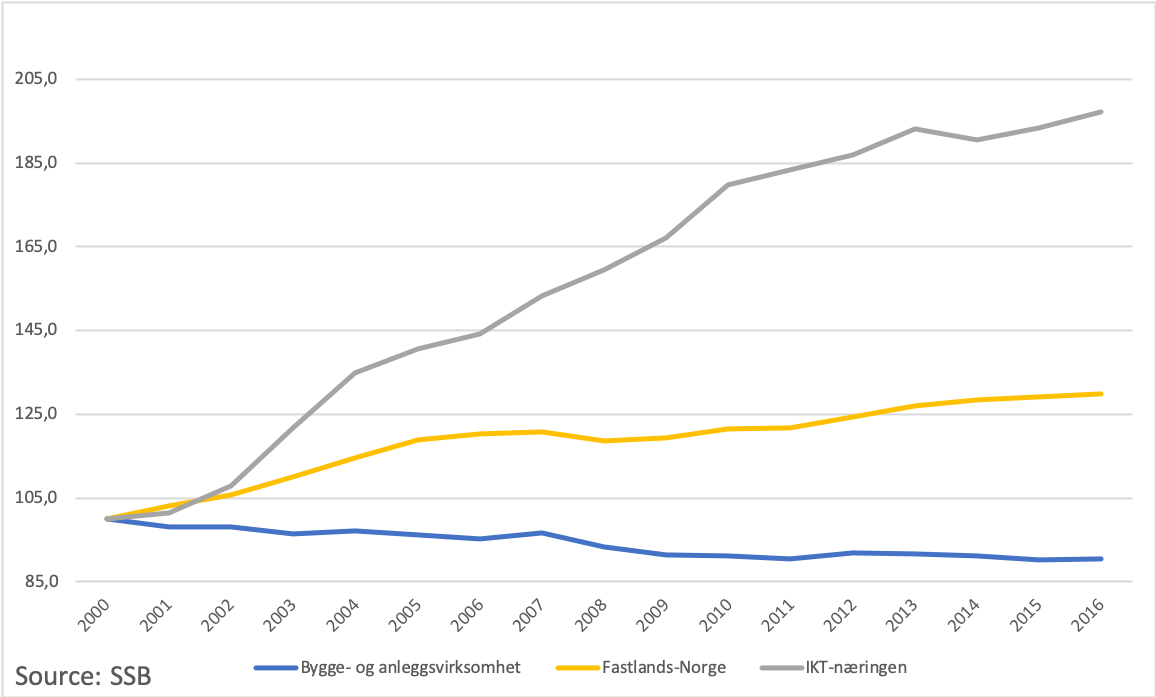
\includegraphics[width=0.9\textwidth]{fig/ba_on-land_ICT.png}
    \caption{Labor productivity in the constructing industry, compared to average on-land industries in Norway, from 2000 to 2016.}
    \label{fig:productivity-comparing}
\end{figure}

\begin{figure}
    \centering
    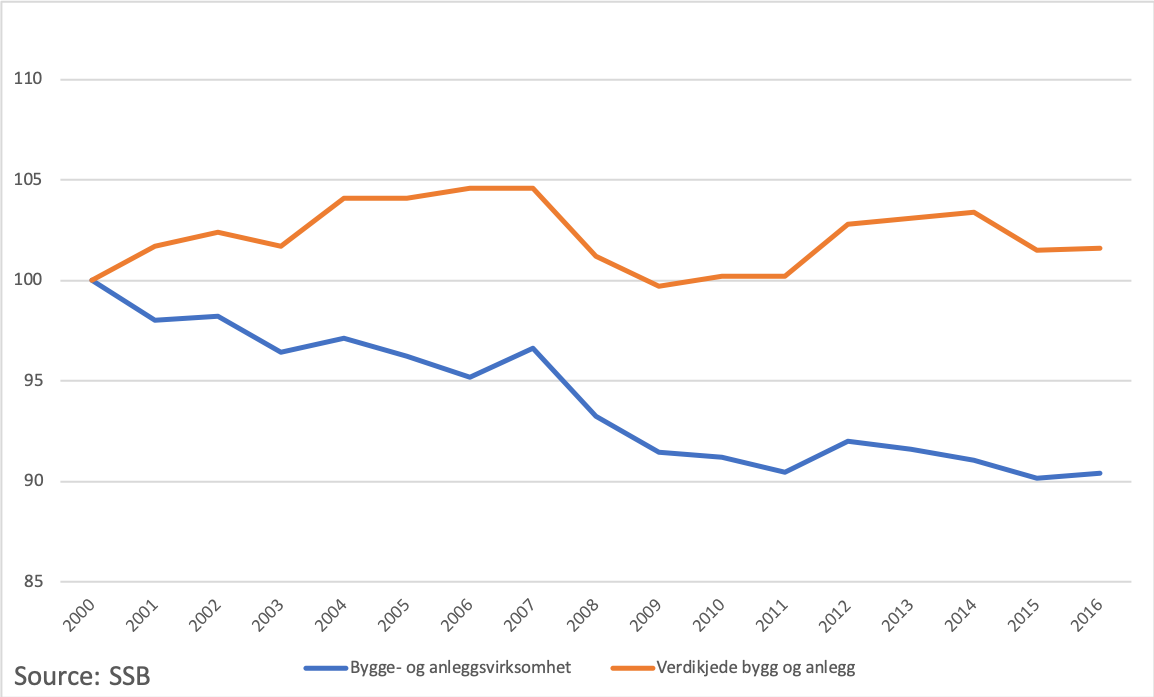
\includegraphics[width=0.9\textwidth]{fig/ba_value_chain.png}
    \caption{Labor productivity in the constructing industry supply chain, from 2000 to 2016.}
    \label{fig:LP_supply_chain}
\end{figure}

An issue paper \cite{langlo2013maaling} posted by Sintef in 2013 raises the discussion about this topic. The issue paper states three central observations: (1) The numbers does not tell the whole story about productivity, (2) the numbers can’t be used in scientific research and (3) the numbers can not be used in comparing businesses, projects or corporations, because each project is so vastly different from one another. 

Looking at observation two, stating that the numbers are not to be used, measuring increased productivity in CI overall. We need, therefore, to look at a process, a specific project, or a corporation to conduct a sufficient scientific analysis. This holds for a case study, where one looks at an individual project, analyzing the internal processes and project management to identify the measurements taken to boost internal productivity. Moreover, complexity makes for no comparison between different projects, because when creating a complicated construction, sometimes new invention needs to happen, and this is not something to be compared. In the same way, comparing productivity in different software development projects is not relevant. If one is to construct the same house, or the same piece of software, time after time, then a comparison is very legit. Then again, in this case, the ingenuity is discussable.

Stating that CI has declining LP is therefore not unilaterally correct - still, if we consider the total value chain, the result is considered poor. The industry is taking action to get LP closer to the average rate. The focus is to make each project as efficient and productive as possible, but that is always the case. Simply because of the marginal cost gained.

Thus yields for a bottom-up approach: Starting with a process in a project and perfecting it, continuing with each process will eventually lead to a resulting better efficiency and productivity in the entire project.  Which, if done in the entire constructing industry, will lead to increased LP overall. Therefore, the industry needs to overcome the challenges, mentioned earlier, (starting with a breach of planned timeline and budget, with symptoms such as requirements change during design, increased complexity, and struggling to complete the products,) were digitalization, Agile (hereunder Lean), is promising and populare solutions to the problem. 


\subsection{Building Informantion Modeling} \label{sec:bim}
BIM is of many seen as a significant contribution to increasing productivity in the CI \cite{frank_gehry, das2014bimcloud, chuang2011applying}. Statsbygg defines it as follows \cite{lean_i_praksis}:

\quad {\bf B} = Building

\quad {\bf I} = Information

\quad {\bf M} = Modeling (Process) or Model (the product) 

The introduction of BIM implicates a significant change, not only in software with three-dimensional models, but also in the workflow and the process \cite{azhar2012building}. With a common model shared among all stakeholders, BIM integrates all disciplines throughout the construction process. What differs BIM with traditional 2D- and 3D-modeling (CAD) technologies? The traditional technologies offered a view of the model, with its dimension in either 2D or 3D. Such as plans, sections, and elevations. If one of these views require for a change, every other view is needed to be checked and updated. Also, these models only showcase entities such as lines, boxes, and circles. Whereas BIM keeps the same traditional view but includes its physical and functional characteristics. In the BIM-model, every element and system is defined as walls, sockets, tubes, and valves. Thus, a single entity in the model, such as a socket, could include dimensions, name, manufacturer, price, and ID. BIM is, in practice, a large relation database, where every entry is defined by a set of core information, with different foreign keys to specific information about the object. Different software providers keep their BIM data in different file formats, but \texttt{.ifc} is a common non-propriety file format, which is shared among most BIM software suppliers.

Introducing BIM is, as mentioned, influencing the process and the workflow of construction. Figure \ref{fig:BIM_process}, illustrates the difference between a traditional (old) process of construction versus the BIM (new) process. 

\begin{figure}
    \centering
    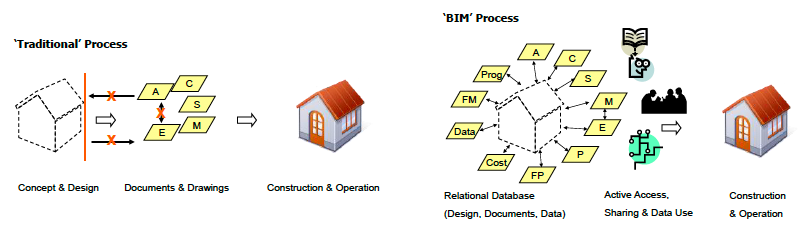
\includegraphics[width=\textwidth]{fig/bim_process.png}
    \caption{A comparison between traditional and BIM construction process. (Courtesy of: Holder Construction, Atlanta, Georgia, USA)}
    \label{fig:BIM_process}
\end{figure}

3D modeling is an essential tool in construction engineering. Since the introduction of 2D data generated drawings (CAD), the evaluation has been rapid. Frank Gehry's introduction of 3D in the Peter B. Lewis building is, by many, the birth of 3D modeling in the construction business. This introduction led to a burst of innovations due to the complex construction, and the visual context 3D modeling gave the engineers \cite{frank_gehry}. The evolution of BIM has been tried synthesized by many \cite{liang2016development}. Figure \ref{fig:bim_levels} is commonly used representation by Bew and Richards \cite{bew2008bim}. Level 3 is where one wants to be nowadays, but most are still at level 2. The difference is in the level of interaction between actors and how they can use a shared model. A distorted BIM model eventually leads to a distorted construction process. Moreover, if the coordination and interaction between disciplines are not in place, the model will eventually fail and lack much information. Hence, the process of BIM. 

The BIM process includes the whole lifecycle of the construction, from programming to demolition, represented in figure \ref{fig:construction_lifecycle}. It is clear to see the utilization of BIM in the Programming- and Design-phase, where architects and engineers create a digital model of the construction to build. Furthermore, in the Construction-phase, the drawings are utilized in the installation and construction of the building.  It is, though, in the last phases of the construction lifecycle that BIM is outstanding. Since the BIM model includes all the data about every system and element of the structure, a caretaker can easily follow up systems and fix an element with the exact products used in its origin. Furthermore, if demolishing a building, BIM can be used to secure this process by identifying every system and element in the building needed to be removed before takedown. 

\begin{figure}
    \centering
    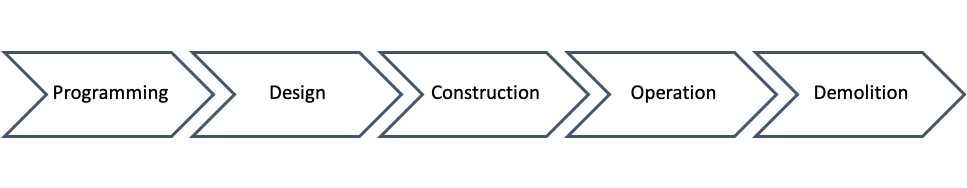
\includegraphics[width=0.75\textwidth]{fig/construction_processes.png}
    \caption{Phases in the construction lifecycle.}
    \label{fig:construction_lifecycle}
\end{figure}

Even though the process of using BIM should promote productivity and interaction between disciplines, this is not easily done in practice \cite{hartmann2012aligning}. The traditional way of working, in silos, still influence the construction business. Aiding the BIM process, several methods and processes have been developed. One is the model maturity index (MMI = Modell Modenhets Indeks) \cite{floisbonn2018mmi}. This index, seen in figure \ref{fig:mmi}, make sure the model is in the correct level detail throughout the project. Also, making sure different actors uses the same language and know what to expect from each other during different phases of the project.

\begin{figure}
    \centering
    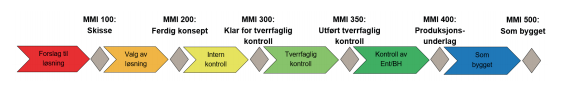
\includegraphics[width=0.8\textwidth]{fig/mmi_process.png}
    \caption{MMI with different stages of the construction process.}
    \label{fig:mmi}
\end{figure}

For a project to utilize BIM, the organization's software is critical. The goal is for the project to include all drawings from all disciplines into a central model. This central model makes for a better flow of information throughout the project \cite{nitithamyong2006success}. A neat feature of BIM is the possibility of collision controls. Collision control is the act of checking if there is any collusion between the different objects in the drawings. Thus, reducing the chance of conflict later in the process. 

Every discipline has its preferred software conducting the modeling. Thus, the diversity of software in BIM is substantial. By Norwegian law, an owner can not dictate which tools to be used in a project. What can be dictated is that every tool to be used in the BIM sphere should be able to produce and read files of the IFC-format. Cloud technology has made it easier to access the BIM model everywhere \cite{azhar2012building}. This access is the case in the shared model, put together by the models of every discipline. For the most part, every discipline and modeler work on their own, using their preferred tool. Thus, the data is stored on their local computer until exported and put together in the shared model. Using BIM promotes cooperation, and using Cloud-based BIM communication is shown to be a cost-effective implementation \cite{das2014bimcloud}, also cloud-based BIM technology is the next step in the BIM evolvement to improve the efficiency of BIM \cite{wong2014review}. The problem is that still, a considerable amount of data is not shared; hence the data stored on the local computer. Autodesk BIM 360 is a platform collecting all relevant disciplines with a shared platform, which includes risk management, procurement, design, and more—using a Software-as-a-Service solution, which makes for effortless view and manipulation of the model. 

Designing in a web browser, using a Software-as-a-Service,  is shown to be complicated. The main issue is the high demand for usability \cite{chuang2011applying}. Thus, most users tend to stick to local computer software.

\begin{figure}
    \centering
    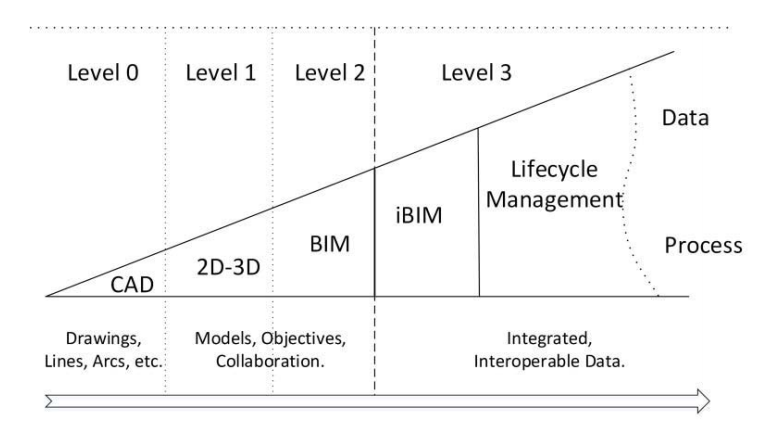
\includegraphics[width=\textwidth]{fig/bim-diagram.png}
    \caption{BIM Maturity Diagram \cite{bew2008bim}}
    \label{fig:bim_levels}
\end{figure}


\section{Agile Project Management}
This section will give an overview of Agile in the context of project management, as well as provide an introduction of different Agile management methods as context for the reader. Furtheremore, a discussion of Agile as a management method, and if the introduction of Lean is in fact just a hype. 

First, when discussing this topic, project methods need to be defined. Different from the \textit{process}, which is more concerned about the different phases of the project, the \textit{method} is about how one can manage within a given stage of a project. Thus, project management methods are about making the most effective utilization of resources within a given phase. 

\subsection{The Motivation for Agile Project Management}
In the ICT-industry the urge for change in project management within distinct phases of projects led to the introduction of agile software development. The move was motivated by having a way of handling late requirements and the growing amount of documentation needed in the ever-more-complex projects. Furthermore, utilizing testing, that way, bugs can be fixed during production, when most uncomplicated. Pushing was also the headlines describing yet another software project failing to meet the schedule. All these symptoms made the software industry move into using agile software development methods as a basis for their project management, starting at the beginning of the '90s and has since been introduced in most software development developments, where needed.  

As we have mentioned increasing productivity and efficiency in a project is desirable for every project, hence marginal cost. This added to the fact that LP in the CI is decreasing made the industry wanting to take action. This project is, therefore, concerned about the bottom-up approach securing more cost-effective and labor-productive management, leading to a more solid industry in the end. The LP-problem is not the only motivation for CI to utilize Agile project management methods. One can identify most of the same issues ICT had when introducing Agile. Most present, as mentioned, is: (a) increased complexity, (b) extensive documentation, (c) reporting of issues leading to change of design during production, and last (d) delivering a construction without errors.

\subsection{Agile Project management}
Seen the motivation for both the ICT and CI to make changes and introduce APM. This section will give a short introduction to APM: the bases as well as some disussion of the use. Furtheremore, the section will introduce some known ASDs, as context for the reader. These methods promote smaller teams of 5-12 people; therefore, included is also an elaboration of ASD in large scale corporations, as well as, Lean, which encourages comparison between SD and Construction. 

APM diverse from linear processes; by the way, a project, or the workers, can rapidly adapt to circumstances. This lines with the problem of requirement change in SD. Moreover, it corresponds to the reporting of issues during production in the CI. The initiatives done since the adaptation of agile in SD was expressed in the Agile Manifesto \cite{agile_manifesto}, when published in 2001. The manifesto gave a tangible reference for project leaders, as well as developers, to steer the project with the correct mindset and focus. Moreover, the manifesto gave a baseline for creating new and potentially better APM methods. The Agile Manifesto says:
\begin{quotation}
    \noindent {\bf Individuals and interactions} over processes and tools \\
    {\bf Working software} over comprehensive documentation \\
    {\bf Customer collaboration} over contract negotiation \\
    {\bf Responding to change} over following a plan \\
\end{quotation}
Including these four sentences, the manifesto also includes a set of twelve principles. Theses principles emphasize always having a working product, an enjoyable working environment, and a proper dialog with the customer. Wich eventually results in a team able to adapt to change,  also late in the development. The manifesto emphasize that face-to-face conversation is the best way of proper conversation, even though much of the interaction can be supported by software.

\subsection{Agile software development in smaller teams}
The above mentioned agile manifesto, says a lot about principals and values when conducting APM and ASD. The manifesto says nothing about the actual process, that is for the different agile methods to explain. Known methods such as SCRUM \cite{sutherland}, Extreme Development (XP) \cite{Beck:1999:EPE:318762}, and Feature-Driven Development\cite{palmer2001practical} are among other descriptions and practices on how to implement scrum as a work method. Abrahamsson, identify that common for all is that they are incremental, straightforward, cooperative, and adaptive \cite{abrahamsson2017agile}. Different from the waterfall process, Abrahamsson concludes, agile emphasizes on being people-centric. 

A generic view of the agile method is iterative development, seen in figure \ref{fig:agile_iteration}. Using the example of SCRUM, the iteration involves sprint-planning, implementation, and review. The method emphasizes growing the team, and after every iteration, a retrospective meeting is being held. Also, worth mentioning is the daily scrum, a meeting where the team discusses the progress, and issues can be raised. Most of the artifacts and events applied in SCRUM has comparable ceremonies in other ASDs. 

\begin{figure}
    \centering
    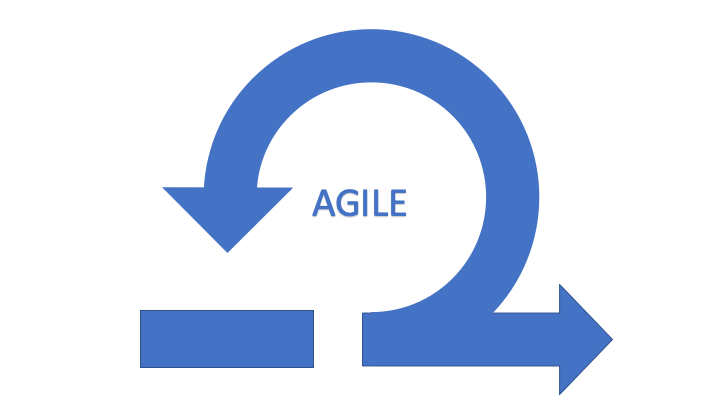
\includegraphics[width=0.8\textwidth]{fig/agile_loop.png}
    \caption{Illustration of the generic agile loop.}
    \label{fig:agile_iteration}
\end{figure}

Still, the process of creating a product has to involve more than just sprint planning. Most of the agile methods also include prior planning before the iterations start. This planning is to be found both in XP and SCRUM. When agile development methods are applied, a problem with estimation often occurs \cite{lang2013cost}. This problem is very present for the managers \cite{dybaa2008empirical}. Traditional project managers utilize a Gantt chart, scheduling project tasks. Sutherland, on the other hand, argues the use of Gantt is mostly a waste of time:
\begin{quote}
    \textit{The only problem with them is that they are always, always wrong.}
\end{quote}
Even though most of the methods encapsulate planning in the process, Abrahamsson, in his paper \cite{abrahamsson2017agile}, discovers that there are only two of the methods implementing concept creation in the process. This is an essential part of the CI project process. Still, one can argue that this is not a part of the development and is supported by the SSA e-procurement process \cite{e-procurement-process}. 

Agile methods are, as the title of this sub-section implicates, planned for smaller teams. Challenges, when extending the team-size, of more than the recommended 5-12 people, are decision-making, communication, and control \cite{xu2009coordination}. Also, when wanting to use the methodologies in large organizations, some adjustment is needen. This made for the introduction of large-scale agile organization methodologies discussed in the next sub-section.  

\subsection{Agile in Large Scale Organizations}
As mentioned, most agile methodologies are designed for smaller teams. Challenges applying agile in large-organization are mostly communication and coordination \cite{dingsoyr2013research}. These issues are well-known when considering large organizations, but are very present when the agile mindset emphasizes harmonization between different actors \cite{miller2002harmonization}. 
When considering large-scale agile, one often want the whole organization to utilize agile with diverse teams. Understanding the concept of agile methodology is problematic. This applies to the managers, and team-members not known to agile beforehand \cite{svorstol2017tailoring}.

When considering large-scale agile organizations, one can divide between organizations using consultants and large in-house scale organizations. When considering projects and organizations of that size, the complexity of management is very present. Still, most of the problems are the same, including knowledge sharing, clear practices, and interacting \cite{smite2019spotify}. In the case of Spotify, they promote continuously improving their practices, as well as communicating in a face-to-face fashion.

Often directors tend to employ old tools and practices not suited for agile, such as Gantt charts, detailed plans and documentation, and set-dates for production \cite{benjaminsen2019}. Both in the case of Spotify and the A-team-project, the discovery is that autonomous team is way more effective than typical teams managed by some leader. Thus, the managers and directors are to facilitate the best infrastructure for the teams. 

\subsection{Lean}\label{sec:lean}
As we know, the term agile was first introduced by Takeuchi and Nanaka in the article \textit{The new new product development game}. They explained how Toyota utilized agile methodology in its construction line. Moreover, the systems used at Toyota are formally named Lean manufacturing and was developed by Ohno and Shingo \cite{becker1998lean}. The idea of the build-measure-learn loop has later been adopted by many other industries, especially after the international bestselling book: \textit{the lean startup} \cite{ries2011lean}. The constant focus on added value to the product is a quintessential aspect of the methodology, which is yearned for many managers out there. 

The lean startup was written by Eric Ries, which origin is software developer, and the approach explained in the book is, therefore, primarily suited for software startups. The act of creating a minimum viable product is not as applicable in the CI. Lean thinking, on the other hand, could still be beneficial for the CI \cite{owen2006agile}, thus leading to the introduction of Lean Construction. 

The cornerstone in Lean thinking is adding value and eliminating waste. Therefore, identifying what is defined as waste and what is value-adding is essential. For example, the CI suffers a significant waste problem. 30\% of construction, in the UK, is rework. In Australia, the number is 35\%. \cite{aziz2013applying}. 

\subsubsection{Lean Construction}\label{sec:lean_construction}
Agile Construction origins from the Lean Manufacturing, and share many mutual ideas, despite operating on vastly different products \cite{salem2006lean}. While in manufacturing, one can move the product around, the physical size of a construction project induce other measures in Constructing. That is why Lean Construction has rejected many of the ideas from Laan Manufacturing \cite{howell1999lean}. 

Applying Lean Thinking in the CI is hence different. Thus, to gain maximum benefit from the lean methodology, there are five fundamental principles to follow proposed by Aziz\cite{aziz2013applying}: 
\begin{enumerate}
    \item {\it Specify Value:} Specify value from customer's own definition and needs and identify the value of activities, which generate value to the end product;
    \item {\it Identify the Value Stram:} Identify the value stream by elimination of everything, which does not generate value to the end product. This means, stop the production when something is going wrong and change it immediately. Processes which have to be avoided are miss production, overproduction (repeat production of the same type of product, etc.), storage of materials and unnecessary processes, transport of materials, movement of labor workforces and products, and finally production of products which does not live up to the wished standard of the customer as well as all kind of unnecessary waiting time;
    \item {\it Flow:} Ensure that there is a continuous flow in the process and value chain by focusing on the entire supply chain. Focus has to be on the process and not at the end product. However, the flow will never get optimal until customer value is specified, and the value stream is identified;
    \item {\it Pull:} Use pull in the production and construction process instead of push. This means produce exactly what the customer wants at the time the customer needs it and always prepared for changes made by customer. The idea is to reduce unnecessary production and to use the management tool "Just In Time";
    \item {\it Perfection:} Aims at the perfect solution and continuous improvements. Deliver a product which lives up to customer's needs and expectations within the agreed time schedule and in a perfect condition without mistakes and defects. The only way to do so is by having a close communication with the customer/client as well as managers, and employees are between.
\end{enumerate}

The essential aspect of Agile Construction is flow. For the method to accomplish the perfect flow, it does, as in other Agile methodologies, stack each iteration with a clear set of objectives to be conducted in the planned timeframe, and the flow is kept by planning the correct amount of tasks before the set deadline. The Norwegian Lean Construction translation uses a train as an image of the flow. Where the idea is for the train to move through the construction. The movement happens when every task within a specific area is completed. The train is represented with a set of carts, each a representation of a discipline. Alining the carts, so that the correct disciplines are in succeeding order.

The output of every flow is the percent planned completed (PPC). The managers can adjust the order of carts, or the number of tasks to make the production more efficient. When utilizing Lean Construction, a top-down approach recommended \cite{lean_i_praksis}. This emphasizes the problem raised by Ingvaldsen, in her article, that the teams lose autonomy when applying Lean in, which conflicts with the Norwegian working model.

\subsubsection{Measuring productivity on project-, process- and process level}
Lean is an excellent method but offers no mechanism measuring the achieved improvements, such as the burndownchart in SCRUM \cite{sutherland}. Skappel, in her master thesis \cite{KPIs_in_lean}, suggests using KPIs measuring the improved perfomence. 
These KPIs are yet to be tested, but still promising ensuring LP in the first phase of a traditional CI-project evolve in the appropriate direction. 

In addition, by recommendation of a issue paper \cite{langlo2013maaling}, a project started in 2015, establishing a state-of-the-art performance measurement tool. In 2017 the resulting Nordic 10-10 \cite{nordic-10-10} program was finished. Nordic 10-10 is a version of the CII 10-10 program\cite{CII-10-10}, designed and translated for the Nordic countries. The CII 10-10 program is a survey-based measurement tool based on the concept of anonymously surveying members of a project, regarding their project's performance, team dynamic, and organizational relationship. The surveying is done at the end of each of the five faces of the constructing project. Opposite to a standard approach, where such analysis is done only one time; at the end of the project. Using Nordic 10-10 results in more agile project management, where changes are implemented throughout the project. In some projects, they even do the analysis even more often, allowing the project manager to make changes also within each phase of the project. 

\subsection{Agile, a populare fade in management?}
Over the past decades, many new trends in project management have emerged and later faded away. A paper \cite{padalkar2016six} exploring six decades of project management trends illustrates the different perspectives of project management. Every trend argues its sovereignty. This illustrates the argument of Rolfsen, in her chapter in the book \textit{Key Issues in Organizational Communication} \cite{rolfsen2004tyranny}, stating that managers are slavish following new fashions of project management. Rolfsen argues that the project management literature is a significant industry of its own. Often the literature is the one answer to every problem and criticizes the older theories, often written using pathos influencing the reader. Even though the literature promotes new methods into the organization, Rolfsen emphasizes that every fade has some good points. 

Even though the focus on different fades promotes different ways of management, the goal is always the same; boost the marginal cost. The results of applying agile in the ICT-industry are promising, hence the increased LP over the past decades. The effect utilizing lean construction, on the other hand, is not to be seen in the statistics, though some papers can report on increased LP \cite{aziz2013applying, ballard1994implementing}.

Applying agile and lean has, for the most part, had a positive impact on projects. Also, every project management trend bring good points into the organization. The deployment of agile is, as mentioned, a way for managers to control the production. Moreover, a tool to control a phase of the process, that has to do with designing and implementation. Added to the process management, the coordination of people in a complex organization is equally as important. The next section is going to discuss this multifaceted area of administration.

\section{Cooperation in Large Organizations}
The work of constructing a highly complex and costly structure is, as we have understood, difficult. There is no straightforward way of doing it, and the focus on project management is an essential part of it. Though, in the end, the act of design and project management is primarily making people work together. Make people interact, coordinate, and synchronize for them to create something that could not happen, if not cooperating. The challenge of making people meet and work together on a common goal, not being self-centered, is something the industry finds difficult. It is seen both in CI, in ICT, and most other industries that have to coordinate different domains of competence. 

This section will discuss this challenge and examine what are the ground principals of cooperation and look at different measures one can make. How may computers support cooperative work? Furthermore, how do contracts influence the interest of different actors to cooperate? 

First, a short introduction to cooperation: Cooperation is the act of communicating and share knowledge in a way that makes different actors coordinate, interact, and synchronize. The act of talking starts with a desire, or at least a reason, for various individuals to talk. 

One must take for granted that the will is there, but in some cases, contracts, politics, or even physical barriers hamper this to happen. Regarding physical barriers, the internet and telecommunication have been a significant leap towards decreasing the boundaries. Computer-supported cooperative work (CSCW) is how technology supports teams cooperate in a project. CSCW will be discussed later in this section. Furthermore, this section will give a brief insight into Norwegian CI- contracts and politics as a context on how for the project, which is an import backdrop for why individuals and parties act the way they do. 

\subsection{Comunication and Knowledge sharing}
The act of talking among project actors and team members is, in most cases, sharing knowledge. One often divides knowledge into tacit- and explicit knowledge. Tacit knowledge is something that is known to actors, but not written down, or otherwise, for somebody else to learn and understand. Where, on the other hand, explicit knowledge can be assimilated simply by reading a manual, or a document. 

A known problem in the CI is knowledge sharing. The motivations for knowledge sharing is as Dainty describes mostly social \cite{dainty2005hrm}. The contractors do what others do, are following the leaders' example, and the feeling of taking part in something bigger than their problems is vital for making people share knowledge. Also, the fact that people need to get something in return when sharing \cite{zhangAttitude}. They get a positive effect through feedback and the effectiveness of their work. Furthermore, Zhang and Ng note that the problem causing people not to share is the fear of losing face. For the managers to contribute to knowledge sharing, they have to create a strategy of capturing and distributing the knowledge \cite{kamara2002knowledge}, often tacit, created in each project.  

Systemizing could help digest explicit knowledge because sometimes the information is there, but how to find it could be the impediment. In modern times computers are taken in to use, systemizing knowledge. Then again, the introduction of computers leads to new tacit knowledge, on how to use the systems. A platform for knowledge sharing could serve positive for the different CI-businesses \cite{kivrak2008capturing}. 

Boundary Objects, introduced in the original paper \cite{star&griesemer}, is a helpful tool when looking at complex situations. Defining objects where actors cooperate and exchange tacit- and explicit knowledge. A boundary object is part of the social world and is, in some way, a facilitator for communication between actors. Star and Greisemer argue that it has to be well-defined, as well as fluid, such that it can both adapt and maintain a collective identity between parties. An example in an engineering project would be documentation or a user manual, which contains explicit knowledge for different parties to share. Furthermore, a stand-up meeting in Lean Construction is a boundary object which emphasizes tacit knowledge sharing.

\subsection{Computer-Supported Cooperative Work}
Computer-Supported Cooperative Work, first defined by \cite{Friedman}, is the theory of the technology's role in the work environment. Often considered in the same context is groupware. The artical \textit{Computer-supported cooperative work: history and focus} \cite{Grudin} describe the motivation for groupware: 
\begin{quotation}
    \noindent \textit{"The complexity of managing large government software contracts provided further incentive to apply technology to group work."} - Jonathan Grundin
\end{quotation}
This motivation applies to Software development as much as for CI. Software and applications as boundary objects have aided complex working groups for centuries. One of the most known, and by Kraut in \cite{Kraut} described as the only successful, CSCW application is e-mail. Groupware has been an essential part of collaborative work, but what makes good groupware? 

To make groupware work, first, it needs to meet the needs and requirements of the group \cite{subramanyam2010user}. When the software is thoroughly developed and tested to meet the requirements, one can argue that the software should work. Still, after a proper software development process, the critical implementation phase begins. Implementing new software has to fit the users. The article \textit{Transforming Work Through Information Technology} by \cite{Robey&Sahay}, describes how the deployment of new groupware in two different counties, ends in two different experiences. Central in the succeeding county, is knowledge sharing and grooming of users beforehand. They were conducting the implementation of the software in a bottom-up manner. In this case, the users were the ones who initiated the deployment. In the other county, who did not succeed, initiating the implementation was a centralized data processing department. As well, the knowledge had to be thought through manuals and learning by doing.

CSCW could also aid knowledge sharing \cite{monplaisir2002enhancing}, by, for example, make use of decision-making software. This way, teams having trouble making decisions can have a trusted source guiding the conclusions. Moreover, the use of ai and big data in the context to support the teams, in ways never seen before, shows promising results, when the ethical issues  \cite{jung2017computational} are kept within boundaries.   

% TODO: Fill out og skrive om til eget språk
For any given individual, it not worth participating unless there is already a sizable group of people participating \cite{grudin1989groupware}. For communication systems and other CSCW systems with similar characteristics, this“critical mass” problem is often a barrier to starting up usage \cite{markus1987toward}.

In the end, to be highly successful, when fulfilled all other terms, the application has to be usable. The software could still work, but often a lot of knowledge is needed to understand the technology, if not emphasizing on high usability. 

\subsection{Contracts in the Construction Industry}
This section will give an introduction to issues concerning contracts in the CI. First, a short introduction to contracts in the CI, as a context for the project. 

\subsubsection*{Contracts in Construction Industry as a Context for the project}
When considering how contractors work together, one has to review the contracts and the politics related. In CI and other fields where contractors are needed, the process outline, defined by SSA, often outlines how to work. During this process, in CI, the party announcing procurements creates tailor-made contracts based on the Norwegian Standard (NS), e.g., NS 8405, NS 8406, NS 8407, and others, which do not support an agile process. This yields a waterfall process. 

Tailor-made deals makes for a challenging space of agreements for the entrepreneurs. This space promotes larger companies or the ones who specialize in contracts from only a few vendors. A contractor who wants to earn a new principal has to learn the contract, giving the advantage to the more experienced contractors. Often the more advanced companies are not pleased when parties introduce new contract outlines - simply because they lose their edge. 

In step 4, the procuring of entrepreneurs phase of the procurement process. In this step, one has to choose an essential element of the contracts, namely, who is responsible. There are two fundamental forms of contracts: (1) Implementation Contract (\textit{Utførelsesentreprise}): where the contractor is answerable for the implementation; and (2) Total Contract (\textit{Totalentreprise}): where the contractor is answerable for both the design and the implementation of the construction, which imply the contractor owns the risk. In both of them, there are different ways of implementing contracts with subcontractors. 

Essential in choosing the fit contract is how one expects the contractors to support one another. A deal that supports interaction is necessary when cooperation is crucial. When is not cooperation essential, one may ask? Often when constructing a modular house, where the owner (hereafter named manager) plans everything, repeatedly building the same house. When designing complex constructions, on the other hand, cooperation is highly desirable. 

When constructing a highly complex construction \textit{Utførelsesentreprise} is often chosen. This way, the risk is at the manager. Choosing the right design of the contract is crucial when aiming for a high degree of cooperation. There is three main contract design. Different is how much coordination and progress management the manager is responsible for managing. The contract models are: 

\begin{itemize}
    \item Shared Contract or Contract Management (CM) (\textit{Byggherrestyrt entrepriser}): The manager makes all deals with subcontractors. In some cases, a subcontractor takes the lead on coordination and progress;
    \item Lead Contract (\textit{Hovedentreprise}): The manager signs a lead contractor, which is responsible for a significant amount of disciplines. Furthermore, the manager establishes subcontracts with the remaining disciplines; 
    \item General Contract (\textit{Generalentreprise}): The manager signs a lead contractor, the general contractor, responsible for signing subcontractors, coordination and progress in the implementation;
\end{itemize}

\subsubsection*{Issues Related to Contracts}
Picking the correct contract is vital in securing desired coordination and interaction, but at the same time, it needs to fit the manager's skills and resources. In the end, choosing the right sort of contract can be vital for meeting the budget. The problem with the complex domain of contracts is that managers tend to pick the same contracts \cite{laedre2006procurement}. Even though construction projects often vary from project to project, the procedure of picking the correct contract for the specific project is often not done.

The politics and contracts in a fragmented CI project, with a handful of contractors and sub-contractors, makes for difficulty in cooperation. Issues related to knowledge sharing is, among others, contracts and politics \cite{alashwal2011knowledge} — the issue origins in the fact that every contractor has the goal of maximizing its marginal cost \cite{miller2002harmonization}. This problem is especially problematic in projects consisting of several different companies, such as in complex constructions. Miller, Packham, and Thomas, in the article, also points out the fact that cooperation and knowledge sharing in mixed teams is the cornerstone in APM. This makes Lean in the CI even more complicated when complex contracts and harmonization among team members are taken into a count. 

Furthermore, the considerable cost of mistrust in CI-projects is shown to be a factor in the overall cost of a project \cite{zaghloul2003construction}. When actors are more busy protecting their contract, rather than adding to the team, the advantages of cross-functional teams can be lost.  Also, prior ties could have a significant impact on how team members interact, as described in the paper of Bruvik and Rolfsen \cite{rolfsen}. 
\begin{quote}
    \textit{Positive prior ties can have a substantial effect on the development of trust at the beginning of the project.}
\end{quote}
Furthermore, the paper is concluded by identifying four aspects that can aid interaction and cooperation: (1) a common philosophy, (2) open communication, (3) clear role expectations, and (4) a shared climate of trust. Hence, prior ties will help in establishing these aspects. One can think that negative prior ties will especially defect the second and the fourth aspect. 

\cleardoublepage